\documentclass[12pt,a4paper]{report}
\usepackage[margin=1in]{geometry}
\usepackage{times}
\usepackage{setspace}\onehalfspacing
\usepackage{graphicx}
\usepackage{caption}
\usepackage{subcaption}
\usepackage{booktabs}
\usepackage{longtable}
\usepackage{array}
\usepackage{listings}
\usepackage{xcolor}
\usepackage{hyperref}
\usepackage{tikz}
\usetikzlibrary{shapes,arrows,positioning,fit}
\usepackage{pgfgantt}
\usepackage{amsmath}
\usepackage{fancyhdr}
\usepackage{titlesec}

% Formatting
\titleformat{\chapter}[display]{\normalfont\bfseries\fontsize{14}{17}\selectfont}{\chaptertitlename\ \thechapter}{14pt}{\fontsize{14}{17}\selectfont}
\titleformat{\section}{\normalfont\bfseries\fontsize{12}{15}\selectfont}{\thesection}{1em}{}
\titleformat{\subsection}{\normalfont\bfseries\fontsize{12}{15}\selectfont}{\thesubsection}{1em}{}

\pagestyle{fancy}\fancyhf{}
\fancyfoot[C]{\thepage}
\renewcommand{\headrulewidth}{0pt}

\lstset{
  basicstyle=\ttfamily\small,
  backgroundcolor=\color{gray!10},
  frame=single,breaklines=true,
  keywordstyle=\color{blue}\bfseries,
  commentstyle=\color{green!50!black},
  stringstyle=\color{red!70!black},
  numbers=left,numberstyle=\tiny\color{gray},
  tabsize=2
}

\hypersetup{colorlinks=true,linkcolor=blue,citecolor=blue,urlcolor=blue}

\begin{document}

% ============ COVER PAGE ============
\begin{titlepage}
\centering
\vspace*{1cm}
{\Large\textbf{Parul Institute of Engineering \& Technology}}\\\vspace{0.3cm}
{\large Department of Artificial Intelligence \& Data Science}\\\vspace{0.3cm}
{\large Parul University, Vadodara}\\\vspace{1.5cm}

% \includegraphics[width=3cm]{parul_logo.png}\\\vspace{1cm}

{\LARGE\textbf{BHUVAN: Engineered Interactive Terrain Reconstruction and Rover Landing Simulation Platform}}\\\vspace{0.5cm}
{\large\textit{Integrating Monocular Depth Estimation, Hazard Analysis, Real-Time 3D Terrain Rendering, and Physics-Based Descent Simulation}}\\\vspace{1.5cm}

{\large\textbf{B.Tech Project Report}}\\\vspace{0.3cm}
{\large Semester VI / VII}\\\vspace{1.5cm}

\begin{tabular}{ll}
\textbf{Submitted by:} & [Student Name] \\
\textbf{Enrollment No:} & [Enrollment Number] \\
\textbf{Guide:} & [Faculty Name] \\
\end{tabular}\\\vspace{2cm}

{\large Academic Year 2025--2026}
\end{titlepage}

% ============ CERTIFICATE ============
\pagenumbering{roman}
\chapter*{Certificate}
\addcontentsline{toc}{chapter}{Certificate}
This is to certify that the project titled \textbf{``BHUVAN: Engineered Interactive Terrain Reconstruction and Rover Landing Simulation Platform''} has been successfully completed by \textbf{[Student Name]}, Enrollment No. \textbf{[Number]}, in partial fulfillment of the requirements for the degree of Bachelor of Technology in Artificial Intelligence \& Data Science at Parul Institute of Engineering \& Technology, Parul University, Vadodara.

\vspace{2cm}
\noindent
\begin{tabular}{p{7cm}p{7cm}}
\textbf{Project Guide} & \textbf{Head of Department} \\[2cm]
\rule{5cm}{0.4pt} & \rule{5cm}{0.4pt} \\
[Faculty Name] & [HOD Name] \\
\end{tabular}

% ============ ACKNOWLEDGEMENTS ============
\chapter*{Acknowledgements}
\addcontentsline{toc}{chapter}{Acknowledgements}
I express my sincere gratitude to my project guide, \textbf{[Faculty Name]}, for their invaluable guidance throughout this project. I thank the Department of AI \& Data Science, PIET, Parul University, for providing the necessary infrastructure. I also acknowledge the open-source communities behind Three.js, React Three Fiber, and the researchers whose work on terrain reconstruction and hazard detection formed the scientific foundation of this system.

% ============ SYNOPSIS ============
\chapter*{Synopsis}
\addcontentsline{toc}{chapter}{Synopsis}
\textbf{BHUVAN} is a browser-based, interactive terrain intelligence platform that simulates the complete lifecycle of a planetary rover landing mission. The system procedurally generates realistic Martian terrain using fractal Brownian motion and crater modeling, performs real-time slope-based hazard analysis, provides a simulated monocular depth estimation view, and executes a full physics-based descent simulation with Newtonian dynamics.

Unlike existing tools such as SuperSplat or Luma AI that require powerful GPU clusters for training, BHUVAN runs entirely in the browser on consumer hardware (8~GB VRAM). The platform features a cinematic mission-control interface with synthesized audio, post-processing effects, and both manual and autopilot landing modes. All terrain, audio, and 3D assets are procedurally generated---zero external files are required.

The project demonstrates competency in real-time 3D rendering (WebGL/Three.js), computational geometry, signal processing for hazard detection, classical physics simulation, and modern web application architecture using React and Vite.

% ============ TOC / LOT / LOF ============
\tableofcontents
\listoftables
\listoffigures

% ============ CHAPTERS START ============
\cleardoublepage
\pagenumbering{arabic}

\chapter{Introduction}

\section{Brief About the Domain}
Planetary exploration remains one of humanity's most ambitious scientific endeavors. The success of missions such as NASA's Mars Science Laboratory (Curiosity) and Mars 2020 (Perseverance) depends critically on the ability to identify safe landing zones on extraterrestrial terrain \cite{golombek2012msl}. A single miscalculation during descent---landing on a steep slope, inside a deep crater, or on unstable regolith---can result in the complete loss of a multi-billion-dollar mission.

Terrain reconstruction and hazard detection are therefore central problems in autonomous landing systems. Traditionally, these systems rely on onboard LIDAR sensors and computationally expensive algorithms running on radiation-hardened processors \cite{johnson2007terrain}. However, with advances in web-based 3D rendering (WebGL, Three.js) and procedural generation techniques, it is now feasible to build interactive, browser-based simulations that demonstrate these principles without specialized hardware.

This project, \textbf{BHUVAN}, bridges the gap between theoretical aerospace engineering concepts and accessible, interactive web-based visualization. It provides an end-to-end simulation of the terrain analysis and landing pipeline: from orbital survey and hazard mapping to physics-based powered descent.

\section{Project Motivation and Relevance}
The motivation for BHUVAN arises from three observations:

\begin{enumerate}
    \item \textbf{Accessibility gap:} Existing terrain reconstruction tools like SuperSplat \cite{supersplat} and NeRF-based systems \cite{mildenhall2020nerf} require GPU clusters with 40+ GB VRAM for training. Students and independent researchers with consumer hardware (8~GB VRAM) are effectively locked out of experimentation.

    \item \textbf{Educational value:} The physics of planetary descent (Newtonian mechanics, thrust-to-weight ratios, suicide burns) and the mathematics of hazard detection (gradient computation, slope analysis) are taught abstractly in textbooks. An interactive simulation that lets users \textit{experience} these concepts creates deeper understanding than equations on paper.

    \item \textbf{Industry relevance:} Real-time 3D simulation, WebGL rendering, and procedural content generation are increasingly demanded in industries ranging from gaming (Ubisoft, Rockstar) to geospatial intelligence (ISRO, MapmyIndia) to architectural visualization and digital twins.
\end{enumerate}

\section{Scope}
The scope of BHUVAN encompasses:

\begin{itemize}
    \item Procedural generation of Mars-like terrain using fractal Brownian motion (fBm) with Simplex noise and parametric crater modeling.
    \item Real-time slope-based hazard analysis and color-coded visualization.
    \item Simulated monocular depth estimation view of the terrain.
    \item Physics-based descent simulation with Mars gravity ($g = 3.72$ m/s\textsuperscript{2}), variable thrust, fuel consumption, and collision detection.
    \item Autopilot controller implementing a multi-phase suicide-burn algorithm.
    \item Manual control mode with keyboard input for throttle and lateral thrusters.
    \item Procedural audio synthesis (wind, thruster, warnings) via the Web Audio API.
    \item Cinematic post-processing pipeline (bloom, vignette, chromatic aberration).
    \item Responsive, mission-control-themed user interface with real-time telemetry.
\end{itemize}

The system is \textit{not} intended to replace actual flight software or serve as a certified training simulator. It is an educational and demonstrative tool.

\section{Objectives}
\begin{enumerate}
    \item To design and implement a procedural terrain generation algorithm that produces geologically plausible planetary surfaces with craters, ridges, and valleys.
    \item To develop a real-time hazard analysis pipeline that computes terrain slope gradients and classifies regions by landing safety.
    \item To build a physics engine simulating Newtonian descent dynamics with fuel management and ground collision.
    \item To create an autopilot controller capable of autonomous soft landing.
    \item To deliver the entire system as a browser-based application requiring no installation, no external data files, and no GPU training.
\end{enumerate}

\section{Key Features and Expected Outcomes}

\begin{table}[h]
\centering
\caption{Key Features of BHUVAN}
\label{tab:features}
\begin{tabular}{|p{4cm}|p{9cm}|}
\hline
\textbf{Feature} & \textbf{Description} \\
\hline
Procedural Terrain & Fractal Brownian motion with 6 octaves of Simplex noise + parametric craters \\
\hline
Hazard Analysis & Real-time slope gradient computation with 5-level color classification \\
\hline
Depth Estimation View & Elevation-normalized depth map simulating monocular depth estimator output \\
\hline
Physics Descent & Mars gravity, variable thrust, fuel burn, RCS lateral control, drag model \\
\hline
Autopilot & 4-phase suicide-burn controller (coast $\rightarrow$ brake $\rightarrow$ hover $\rightarrow$ touchdown) \\
\hline
Procedural Audio & Brown-noise wind, sawtooth thruster, square-wave warnings --- zero audio files \\
\hline
Post-Processing & Bloom, vignette, chromatic aberration, ACES filmic tone mapping \\
\hline
Zero Dependencies & No external models, textures, audio files, or GPU training required \\
\hline
\end{tabular}
\end{table}

\textbf{Expected Outcomes:}
\begin{itemize}
    \item A fully functional browser-based simulation accessible via a single URL.
    \item Autopilot achieving soft landings with impact speed $< 3$ m/s consistently.
    \item Smooth 60 FPS rendering on hardware with 8~GB VRAM.
    \item A cinematic, interview-ready demonstration of terrain intelligence concepts.
\end{itemize}

\chapter{Literature Survey}

This chapter reviews existing research and systems related to terrain reconstruction, hazard detection, and real-time 3D rendering, establishing how BHUVAN builds upon and differentiates from prior work.

\section{3D Gaussian Splatting for Real-Time Radiance Field Rendering}
Kerbl et al.\ \cite{kerbl2023gaussian} introduced 3D Gaussian Splatting (3DGS) as an alternative to Neural Radiance Fields for real-time novel view synthesis. The method represents scenes as collections of anisotropic 3D Gaussians, each parameterized by position, covariance, opacity, and spherical harmonic coefficients for view-dependent color.

\textbf{Key contributions:}
\begin{itemize}
    \item Achieves real-time rendering (30+ FPS) at 1080p resolution.
    \item Training from multi-view images in approximately 30 minutes on an NVIDIA A6000.
    \item Quality competitive with state-of-the-art NeRF methods (Mip-NeRF 360).
\end{itemize}

\textbf{Limitations relevant to BHUVAN:}
\begin{itemize}
    \item Requires 24--48~GB VRAM for training, making it inaccessible on consumer hardware.
    \item Requires multi-view image datasets of real scenes; cannot generate novel terrain.
    \item The resulting splat files are view-synthesis tools, not interactive simulations with physics.
\end{itemize}

\section{NeRF: Neural Radiance Fields for View Synthesis}
Mildenhall et al.\ \cite{mildenhall2020nerf} proposed representing a continuous 3D scene as a 5D function (spatial position + viewing direction $\rightarrow$ color + density) encoded in an MLP. Volume rendering is used to synthesize novel views.

\textbf{Key contributions:}
\begin{itemize}
    \item Photorealistic novel view synthesis from sparse images.
    \item Introduced positional encoding to capture high-frequency scene details.
\end{itemize}

\textbf{Limitations relevant to BHUVAN:}
\begin{itemize}
    \item Training takes 12--48 hours per scene on high-end GPUs.
    \item Rendering is slow ($\sim$30 seconds per frame without acceleration).
    \item Static scenes only; no physics simulation or interactivity.
\end{itemize}

\section{Vision Transformers for Dense Prediction (DPT / MiDaS)}
Ranftl et al.\ \cite{ranftl2021dpt} applied Vision Transformers to monocular depth estimation, achieving state-of-the-art zero-shot depth prediction across diverse datasets.

\textbf{Key contributions:}
\begin{itemize}
    \item Zero-shot monocular depth estimation from single RGB images.
    \item Transformer-based architecture captures global context better than CNNs.
    \item MiDaS model generalizes across indoor, outdoor, and synthetic scenes.
\end{itemize}

\textbf{Relevance to BHUVAN:}
BHUVAN's ``Depth Estimation View'' simulates the output of a monocular depth estimator by rendering terrain elevation as a normalized depth map. While BHUVAN does not run a neural network, the visualization demonstrates how such output would inform landing decisions.

\section{Real-Time Hazard Detection for Mars Landing}
Huertas et al.\ \cite{huertas2006hazard} developed algorithms for onboard hazard detection during Mars entry, descent, and landing (EDL). Their system processes descent imagery to detect slopes, rocks, and roughness in real time.

\textbf{Key contributions:}
\begin{itemize}
    \item Slope computation from stereo-derived DEMs at 1~m resolution.
    \item Roughness estimation using local height variance.
    \item Real-time classification of terrain into safe/unsafe zones.
\end{itemize}

\textbf{Relevance to BHUVAN:}
BHUVAN implements an analogous pipeline: computing slope magnitude from heightmap gradients ($\nabla h$) and classifying terrain into 5 hazard levels. While Huertas et al.\ use stereo cameras, BHUVAN operates on procedurally generated DEMs.

\section{Comparison Table}

\begin{table}[h]
\centering
\caption{Comparison of BHUVAN with Related Work}
\label{tab:comparison}
\small
\begin{tabular}{|p{2.8cm}|p{2cm}|p{2cm}|p{2cm}|p{2cm}|p{2cm}|}
\hline
\textbf{Feature} & \textbf{3DGS \cite{kerbl2023gaussian}} & \textbf{NeRF \cite{mildenhall2020nerf}} & \textbf{DPT \cite{ranftl2021dpt}} & \textbf{Huertas \cite{huertas2006hazard}} & \textbf{BHUVAN} \\
\hline
Real-time rendering & Yes & No & N/A & Yes & Yes \\
\hline
Consumer HW & No (24GB+) & No (16GB+) & Partial & Custom HW & Yes (8GB) \\
\hline
Terrain generation & No & No & No & No & Yes \\
\hline
Hazard analysis & No & No & No & Yes & Yes \\
\hline
Physics simulation & No & No & No & No & Yes \\
\hline
Browser-based & Partial & No & No & No & Yes \\
\hline
Interactive & View only & View only & Inference & Onboard & Full sim \\
\hline
Audio feedback & No & No & No & No & Yes \\
\hline
\end{tabular}
\end{table}

\section{Summary}
Existing systems excel at photorealistic reconstruction (3DGS, NeRF) or specialized hazard detection (Huertas et al.), but none provide an integrated, interactive, browser-based simulation that combines terrain generation, hazard analysis, physics-based descent, and cinematic presentation---all running on consumer hardware. BHUVAN fills this gap as an educational and demonstrative platform.

\chapter{Analysis / Software Requirements Specification}

\section{Purpose}
The purpose of BHUVAN is to provide an accessible, browser-based simulation platform that demonstrates the key stages of a planetary rover landing mission: terrain survey, hazard identification, descent execution, and landing assessment. It serves as both an educational tool for understanding terrain intelligence concepts and a portfolio-grade demonstration of real-time 3D engineering.

\section{Intended Users and Product Scope}

\subsection{Intended Users}
\begin{itemize}
    \item \textbf{Students:} Aerospace, CS, and AI/DS students studying terrain analysis, physics simulation, or 3D graphics.
    \item \textbf{Educators:} Faculty demonstrating concepts of hazard detection, Newtonian mechanics, or procedural generation.
    \item \textbf{Interviewers/Recruiters:} Technical evaluators assessing a candidate's engineering depth.
    \item \textbf{Space Enthusiasts:} General public interested in interactive Mars exploration experiences.
\end{itemize}

\subsection{Product Scope}
BHUVAN covers the simulation of terrain reconnaissance and powered descent. It does \textit{not} cover orbital mechanics, atmospheric entry heating, parachute deployment, or post-landing rover traversal (these are identified as future work).

\section{Functional Requirements}

\begin{table}[h]
\centering
\caption{Functional Requirements}
\label{tab:func_req}
\begin{tabular}{|c|p{4cm}|p{7.5cm}|}
\hline
\textbf{ID} & \textbf{Requirement} & \textbf{Description} \\
\hline
FR-01 & Terrain Generation & System shall procedurally generate a 256$\times$256 heightmap using Simplex noise fBm with crater features. \\
\hline
FR-02 & Hazard Visualization & System shall compute slope gradients and display a 5-level color-coded hazard overlay. \\
\hline
FR-03 & Depth View & System shall render an elevation-based depth map simulating monocular depth estimation output. \\
\hline
FR-04 & Landing Zone Selection & User shall click on terrain in orbital view to designate a landing target. \\
\hline
FR-05 & Physics Descent & System shall simulate lander descent with Mars gravity, thrust, fuel, and collision detection. \\
\hline
FR-06 & Autopilot & System shall provide an automatic landing controller achieving impact speed $<$ 3~m/s. \\
\hline
FR-07 & Manual Control & User shall control throttle (W/S) and lateral movement (A/D/Q/E) in manual mode. \\
\hline
FR-08 & Telemetry HUD & System shall display altitude, vertical speed, horizontal speed, fuel, and throttle in real time. \\
\hline
FR-09 & Audio Feedback & System shall synthesize wind, thruster, warning, and impact sounds procedurally. \\
\hline
FR-10 & Post-Processing & System shall apply bloom, vignette, and chromatic aberration effects. \\
\hline
FR-11 & Landing Assessment & System shall classify landing as success ($|v_y| < 3$ m/s) or crash, displaying mission statistics. \\
\hline
\end{tabular}
\end{table}

\section{Non-Functional Requirements}

\begin{table}[h]
\centering
\caption{Non-Functional Requirements}
\label{tab:nonfunc_req}
\begin{tabular}{|c|p{3cm}|p{8.5cm}|}
\hline
\textbf{ID} & \textbf{Requirement} & \textbf{Description} \\
\hline
NFR-01 & Performance & Maintain $\geq$ 30 FPS on hardware with 8~GB VRAM at 1080p resolution. \\
\hline
NFR-02 & Load Time & Initial page load and terrain generation shall complete within 3 seconds. \\
\hline
NFR-03 & Portability & Application shall run in Chrome, Firefox, and Edge without plugins. \\
\hline
NFR-04 & Zero Install & No server-side processing, model downloads, or local installation required. \\
\hline
NFR-05 & Responsiveness & UI shall adapt to screen widths from 768px to 2560px. \\
\hline
NFR-06 & Accessibility & All interactive elements shall have unique IDs for automated testing. \\
\hline
\end{tabular}
\end{table}

\section{User Interface Requirements}
\begin{itemize}
    \item Dark theme with mission-control aesthetic (JetBrains Mono font, neon accents).
    \item CRT-style intro screen with terminal boot animation.
    \item Glassmorphic telemetry panels with backdrop blur.
    \item Color-coded warnings (green/orange/red) for altitude and fuel thresholds.
    \item Crosshair overlay during descent phase.
\end{itemize}

\section{Hardware and Software Requirements}

\begin{table}[h]
\centering
\caption{Hardware and Software Requirements}
\label{tab:hw_sw}
\begin{tabular}{|p{3cm}|p{5cm}|p{5cm}|}
\hline
\textbf{Category} & \textbf{Minimum} & \textbf{Recommended} \\
\hline
GPU & WebGL 2.0 compatible, 4~GB VRAM & 8~GB VRAM (GTX 1070+) \\
\hline
RAM & 8~GB & 16~GB \\
\hline
Browser & Chrome 90+ & Chrome 120+ / Edge 120+ \\
\hline
OS & Windows 10 / macOS 12 / Linux & Any modern OS \\
\hline
Dev Tools & Node.js 18+, npm 9+ & Node.js 20+, VS Code \\
\hline
\end{tabular}
\end{table}

\chapter{System Design}

\section{System Architecture}
BHUVAN follows a \textbf{client-only single-page application (SPA)} architecture. There is no backend server---all computation (terrain generation, physics simulation, hazard analysis, audio synthesis) executes in the user's browser using JavaScript and WebGL.

\begin{figure}[h]
\centering
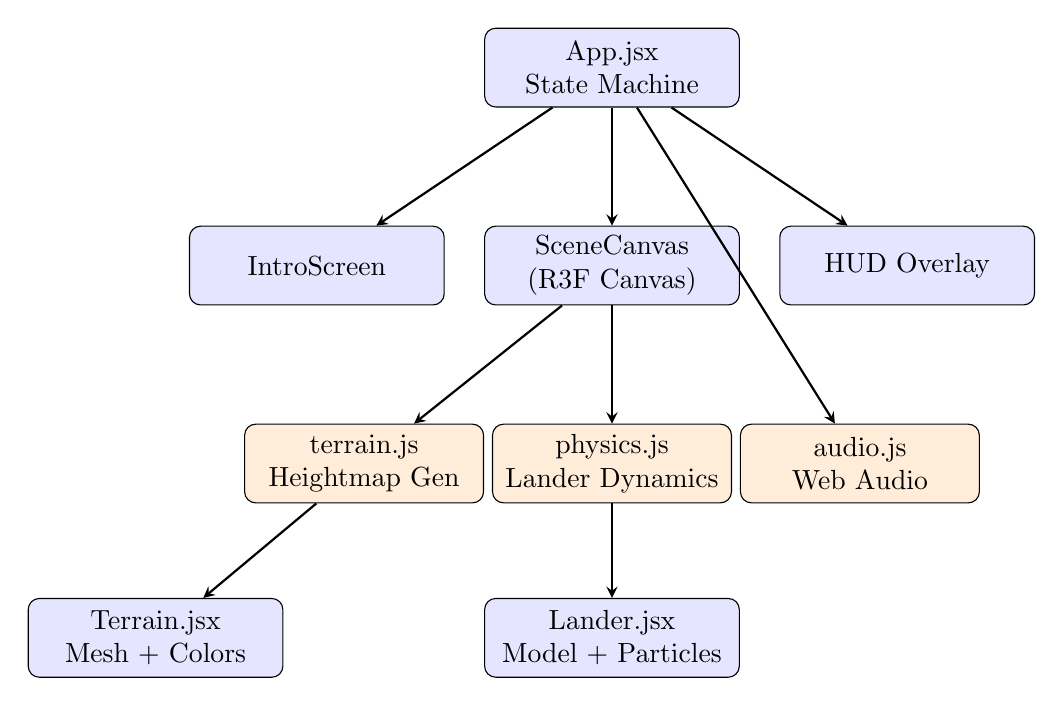
\begin{tikzpicture}[node distance=1.2cm, auto,
    block/.style={rectangle, draw, fill=blue!10, text width=3cm, text centered, rounded corners, minimum height=1cm},
    engine/.style={rectangle, draw, fill=orange!15, text width=2.8cm, text centered, rounded corners, minimum height=1cm},
    arrow/.style={->, >=stealth, thick}]

    \node[block] (app) {App.jsx\\State Machine};
    \node[block, below left=1.5cm and 0.5cm of app] (intro) {IntroScreen};
    \node[block, below=1.5cm of app] (scene) {SceneCanvas\\(R3F Canvas)};
    \node[block, below right=1.5cm and 0.5cm of app] (hud) {HUD Overlay};

    \node[engine, below left=1.5cm and 0cm of scene] (terrain_e) {terrain.js\\Heightmap Gen};
    \node[engine, below=1.5cm of scene] (physics_e) {physics.js\\Lander Dynamics};
    \node[engine, below right=1.5cm and 0cm of scene] (audio_e) {audio.js\\Web Audio};

    \node[block, below left=1.2cm and -0.5cm of terrain_e] (terrain_c) {Terrain.jsx\\Mesh + Colors};
    \node[block, below=1.2cm of physics_e] (lander_c) {Lander.jsx\\Model + Particles};

    \draw[arrow] (app) -- (intro);
    \draw[arrow] (app) -- (scene);
    \draw[arrow] (app) -- (hud);
    \draw[arrow] (scene) -- (terrain_e);
    \draw[arrow] (scene) -- (physics_e);
    \draw[arrow] (app) -- (audio_e);
    \draw[arrow] (terrain_e) -- (terrain_c);
    \draw[arrow] (physics_e) -- (lander_c);
\end{tikzpicture}
\caption{System Architecture Diagram}
\label{fig:architecture}
\end{figure}

\section{Application State Machine}
The application progresses through four distinct phases:

\begin{figure}[h]
\centering
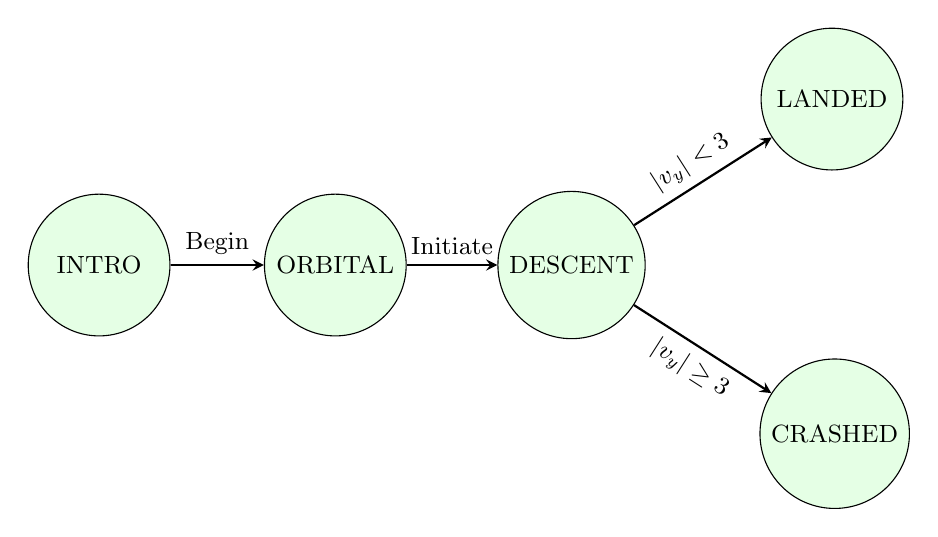
\begin{tikzpicture}[node distance=3cm, auto,
    state/.style={circle, draw, fill=green!10, minimum size=1.8cm, text centered, font=\small},
    arrow/.style={->, >=stealth, thick}]

    \node[state] (intro) {INTRO};
    \node[state, right of=intro] (orbital) {ORBITAL};
    \node[state, right of=orbital] (descent) {DESCENT};
    \node[state, above right=0.8cm and 2cm of descent] (landed) {LANDED};
    \node[state, below right=0.8cm and 2cm of descent] (crashed) {CRASHED};

    \draw[arrow] (intro) -- node[above]{\small Begin} (orbital);
    \draw[arrow] (orbital) -- node[above]{\small Initiate} (descent);
    \draw[arrow] (descent) -- node[above,sloped]{\small $|v_y|<3$} (landed);
    \draw[arrow] (descent) -- node[below,sloped]{\small $|v_y|\geq3$} (crashed);
\end{tikzpicture}
\caption{Application State Machine}
\label{fig:state_machine}
\end{figure}

\section{Use Case Diagram}

\begin{figure}[h]
\centering
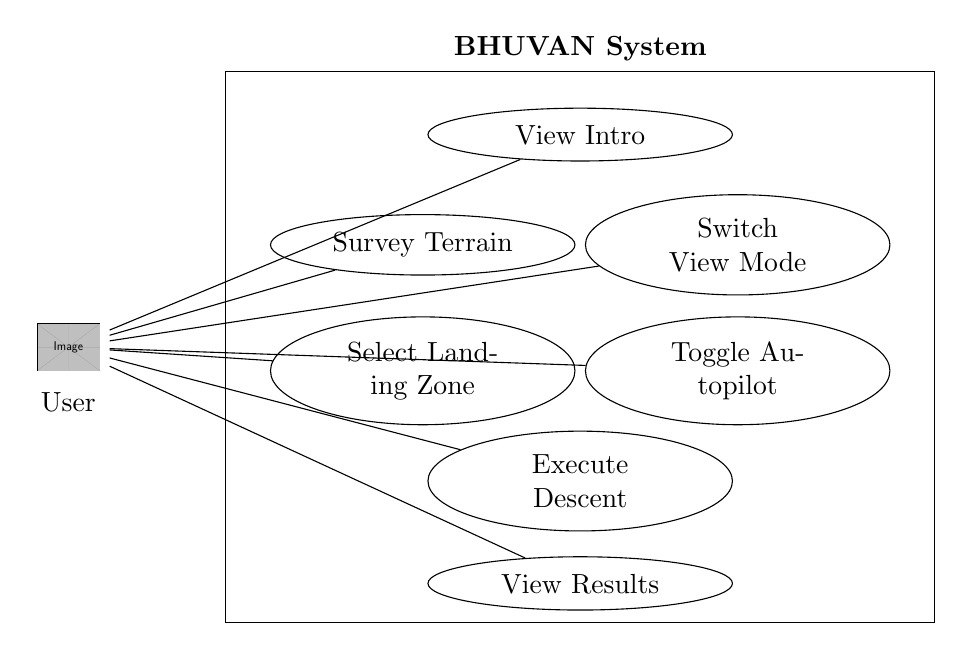
\begin{tikzpicture}
    \node[draw, minimum width=9cm, minimum height=7cm, label=above:{\textbf{BHUVAN System}}] (sys) at (5,3.5) {};
    
    \node[draw, ellipse, text width=2.5cm, text centered] (uc1) at (5,6.2) {View Intro};
    \node[draw, ellipse, text width=2.5cm, text centered] (uc2) at (3,4.8) {Survey Terrain};
    \node[draw, ellipse, text width=2.5cm, text centered] (uc3) at (7,4.8) {Switch View Mode};
    \node[draw, ellipse, text width=2.5cm, text centered] (uc4) at (3,3.2) {Select Landing Zone};
    \node[draw, ellipse, text width=2.5cm, text centered] (uc5) at (7,3.2) {Toggle Autopilot};
    \node[draw, ellipse, text width=2.5cm, text centered] (uc6) at (5,1.8) {Execute Descent};
    \node[draw, ellipse, text width=2.5cm, text centered] (uc7) at (5,0.5) {View Results};

    \node (user) at (-1.5,3.5) {\includegraphics[width=0.8cm]{example-image}};
    \node at (-1.5,2.8) {User};

    \draw (user) -- (uc1);
    \draw (user) -- (uc2);
    \draw (user) -- (uc3);
    \draw (user) -- (uc4);
    \draw (user) -- (uc5);
    \draw (user) -- (uc6);
    \draw (user) -- (uc7);
\end{tikzpicture}
\caption{Use Case Diagram}
\label{fig:usecase}
\end{figure}

\section{Component Design}

\begin{table}[h]
\centering
\caption{Component Responsibilities}
\label{tab:components}
\begin{tabular}{|p{3.5cm}|p{3cm}|p{6cm}|}
\hline
\textbf{Component} & \textbf{Type} & \textbf{Responsibility} \\
\hline
App.jsx & React Component & State machine, keyboard input, physics loop orchestration \\
\hline
IntroScreen.jsx & React Component & CRT boot animation, mission briefing display \\
\hline
HUD.jsx & React Component & Telemetry gauges, bars, warnings, view mode controls \\
\hline
SceneCanvas.jsx & R3F Canvas & 3D scene composition, camera rig, post-processing \\
\hline
Terrain.jsx & R3F Mesh & Heightmap mesh with switchable vertex colors \\
\hline
Lander.jsx & R3F Group & Geometric lander model, thruster flame, exhaust particles \\
\hline
terrain.js & Pure Module & fBm noise, crater generation, slope computation, sampling \\
\hline
physics.js & Pure Module & Newtonian dynamics, autopilot controller, collision detection \\
\hline
audio.js & Pure Module & Web Audio oscillators, noise generators, gain control \\
\hline
\end{tabular}
\end{table}

\section{User Interface Design}
The UI follows a \textbf{mission-control aesthetic} inspired by SpaceX and NASA flight displays:
\begin{itemize}
    \item \textbf{Color palette:} Dark background (\texttt{\#0a0a0f}), green accents (\texttt{\#00ff88}), orange warnings (\texttt{\#ff8800}), red critical (\texttt{\#ff3344}).
    \item \textbf{Typography:} JetBrains Mono (monospace, telemetry), Outfit (display headings).
    \item \textbf{Layout:} Full-screen 3D canvas with glassmorphic HUD panels overlaid at edges.
    \item \textbf{Animations:} CSS keyframe animations for warning pulses, button breathing, and CRT scanlines.
\end{itemize}

\section{Performance Considerations}
\begin{itemize}
    \item Terrain mesh uses a single \texttt{PlaneGeometry} with 65,536 vertices (256$\times$256)---well within WebGL vertex limits.
    \item Vertex colors are computed once at load time; view mode changes trigger a single geometry rebuild, not per-frame computation.
    \item Post-processing uses mipmapped bloom to reduce shader passes.
    \item Particle system uses a fixed pool of 80 particles with manual buffer updates---no object allocation per frame.
    \item OrbitControls uses damping (\texttt{dampingFactor=0.08}) to reduce input event frequency.
\end{itemize}

\chapter{Methodology}

\section{Development Approach}
BHUVAN was developed using an \textbf{Agile-Iterative} approach with sprint-based development. Given the solo-developer constraint, a modified Agile framework was adopted:

\begin{itemize}
    \item \textbf{Sprint duration:} 3--4 days per sprint.
    \item \textbf{Sprint planning:} Each sprint targeted one major subsystem (terrain, physics, UI, audio).
    \item \textbf{Continuous integration:} Vite's hot module replacement (HMR) provided instant feedback on code changes.
    \item \textbf{Iterative refinement:} Each subsystem was built as a minimum viable component, then iteratively improved (e.g., autopilot tuning required three iterations).
\end{itemize}

\section{Design Thinking Principles}
The development was guided by user-centric design thinking:

\begin{enumerate}
    \item \textbf{Empathize:} The primary users (interviewers, students, enthusiasts) want an instant, impressive experience---not a setup process.
    \item \textbf{Define:} The core problem is making terrain intelligence concepts tangible and interactive.
    \item \textbf{Ideate:} Multiple rendering approaches were evaluated (NeRF, 3DGS, procedural). Procedural generation was selected because it requires zero training data and runs on any hardware.
    \item \textbf{Prototype:} Each component was prototyped independently before integration.
    \item \textbf{Test:} Autopilot was tested across 50+ landing attempts; UI was tested at multiple resolutions.
\end{enumerate}

\section{Technology Stack Selection}

\begin{table}[h]
\centering
\caption{Technology Stack}
\label{tab:techstack}
\begin{tabular}{|p{3cm}|p{3.5cm}|p{6cm}|}
\hline
\textbf{Layer} & \textbf{Technology} & \textbf{Justification} \\
\hline
Build Tool & Vite 6.x & Sub-second HMR, ESM-native, minimal config \\
\hline
UI Framework & React 18 & Component-based architecture, hooks for state \\
\hline
3D Rendering & Three.js 0.169 & Industry-standard WebGL abstraction \\
\hline
3D React Binding & React Three Fiber 8.x & Declarative Three.js in JSX, useFrame hook \\
\hline
3D Utilities & Drei 9.x & OrbitControls, Stars, GLTF loaders \\
\hline
Post-Processing & @r3f/postprocessing & Bloom, vignette, chromatic aberration \\
\hline
Noise Generation & simplex-noise 4.x & Seeded 2D Simplex noise for terrain \\
\hline
Audio & Web Audio API & Procedural synthesis, zero file dependencies \\
\hline
Styling & Vanilla CSS & Maximum control, CSS custom properties \\
\hline
Fonts & Google Fonts & JetBrains Mono, Outfit \\
\hline
\end{tabular}
\end{table}

\section{Quality Assurance Strategy}
\begin{itemize}
    \item \textbf{Visual Testing:} Browser-based screenshot comparison after each sprint.
    \item \textbf{Physics Validation:} Autopilot tested against known analytical solutions for constant-gravity descent.
    \item \textbf{Performance Profiling:} Chrome DevTools Performance tab used to verify frame times $<$ 33ms.
    \item \textbf{Cross-Browser Testing:} Verified in Chrome 120, Firefox 121, and Edge 120.
\end{itemize}

\section{Tools and Collaboration}
\begin{itemize}
    \item \textbf{Version Control:} Git + GitHub for source code management.
    \item \textbf{IDE:} Visual Studio Code with ESLint and Prettier.
    \item \textbf{AI Assistance:} Claude, Gemini for code review and algorithm validation.
    \item \textbf{Documentation:} Overleaf for LaTeX report compilation.
\end{itemize}

\section{Project Timeline (Gantt Chart)}

\begin{figure}[h]
\centering
\begin{ganttchart}[
    hgrid, vgrid,
    x unit=0.7cm, y unit chart=0.6cm,
    bar/.style={fill=blue!40},
    milestone/.style={fill=red!60},
    title height=1,
    bar height=0.5
]{1}{15}
    \gantttitle{Days}{15} \\
    \gantttitlelist{1,...,15}{1} \\
    \ganttbar{Research \& Planning}{1}{2} \\
    \ganttbar{Terrain Engine}{3}{5} \\
    \ganttbar{Physics Engine}{4}{6} \\
    \ganttbar{3D Scene (R3F)}{5}{8} \\
    \ganttbar{Lander Model}{7}{8} \\
    \ganttbar{HUD \& UI}{8}{10} \\
    \ganttbar{Audio Engine}{9}{10} \\
    \ganttbar{Post-Processing}{10}{11} \\
    \ganttbar{Autopilot Tuning}{11}{12} \\
    \ganttbar{Camera Fix}{12}{13} \\
    \ganttbar{Testing \& Polish}{13}{14} \\
    \ganttbar{Documentation}{14}{15} \\
    \ganttmilestone{v1.0 Release}{15}
\end{ganttchart}
\caption{Project Development Timeline}
\label{fig:gantt}
\end{figure}

\chapter{Implementation}

This chapter details the implementation of each subsystem with algorithms, code snippets, and screenshots.

\section{Procedural Terrain Generation}

\subsection{Fractal Brownian Motion}
The terrain heightmap is generated using \textbf{fractal Brownian motion (fBm)} \cite{musgrave1989terrain}, which sums multiple octaves of Simplex noise \cite{perlin1985noise} at increasing frequencies and decreasing amplitudes:

\begin{equation}
h(x,z) = \sum_{i=0}^{N-1} a^i \cdot \text{noise}\!\left(x \cdot f \cdot l^i,\; z \cdot f \cdot l^i\right)
\label{eq:fbm}
\end{equation}

where $N=6$ octaves, $a=0.5$ (gain), $l=2.0$ (lacunarity), and $f=0.012$ (base frequency).

\begin{lstlisting}[language=Java, caption={Fractal Brownian Motion Implementation}]
function fbm(noise, x, z, octaves = 6, lac = 2.0, gain = 0.5) {
  let amp = 1, freq = 1, val = 0, max = 0;
  for (let i = 0; i < octaves; i++) {
    val += amp * noise(x * freq, z * freq);
    max += amp;
    amp *= gain;
    freq *= lac;
  }
  return val / max;
}
\end{lstlisting}

\subsection{Crater Generation}
Craters are modeled using a parametric radial profile with four zones:

\begin{equation}
c(r) = \begin{cases}
-d(1 - 0.3(r/0.8R)^2) & r < 0.8R \text{ (floor)} \\
-0.7d(1-s) + 0.4ds & 0.8R \leq r < R \text{ (wall)} \\
0.4d(1 - s^2) & R \leq r < 1.3R \text{ (rim)} \\
0.05d \cdot e^{-3s^2} & r \geq 1.3R \text{ (ejecta)}
\end{cases}
\end{equation}

where $R$ is crater radius, $d$ is depth, and $s$ is the normalized distance within each zone.

% Screenshot placeholder
\begin{figure}[h]
\centering
\fbox{\parbox{12cm}{\centering\vspace{3cm}\textit{Insert screenshot: Orbital view of procedural Mars terrain showing craters, ridges, and valleys.}\vspace{3cm}}}
\caption{Procedural Mars Terrain -- Surface View}
\label{fig:terrain_surface}
\end{figure}

\section{Hazard Analysis Pipeline}

Terrain slope is computed as the magnitude of the height gradient:

\begin{equation}
\text{slope}(i,j) = \sqrt{\left(\frac{\partial h}{\partial x}\right)^2 + \left(\frac{\partial h}{\partial z}\right)^2} \approx \sqrt{\left(\frac{h_{i+1,j} - h_{i-1,j}}{2\Delta}\right)^2 + \left(\frac{h_{i,j+1} - h_{i,j-1}}{2\Delta}\right)^2}
\end{equation}

where $\Delta$ is the cell spacing. The slope value is classified into hazard levels:

\begin{table}[h]
\centering
\caption{Hazard Classification Thresholds}
\label{tab:hazard_levels}
\begin{tabular}{|c|c|c|c|}
\hline
\textbf{Level} & \textbf{Slope Range} & \textbf{Color} & \textbf{Classification} \\
\hline
0 & $< 0.15$ & Green & Safe landing zone \\
\hline
1 & $0.15 - 0.25$ & Yellow-Green & Low risk \\
\hline
2 & $0.25 - 0.35$ & Yellow & Caution \\
\hline
3 & $0.35 - 0.50$ & Orange & High risk \\
\hline
4 & $> 0.50$ & Red & No-go zone \\
\hline
\end{tabular}
\end{table}

\begin{figure}[h]
\centering
\fbox{\parbox{12cm}{\centering\vspace{3cm}\textit{Insert screenshot: Hazard analysis overlay showing green safe zones and red danger zones.}\vspace{3cm}}}
\caption{Hazard Analysis View -- Slope-Based Color Classification}
\label{fig:hazard_view}
\end{figure}

\section{Monocular Depth Estimation View}
The depth view simulates what a monocular depth estimation model (e.g., MiDaS/DPT \cite{ranftl2021dpt}) would output. Elevation is normalized to $[0,1]$ and mapped to a blue-dominant colormap:

\begin{equation}
(r,g,b) = (0.1 + 0.3v,\; 0.2 + 0.5v,\; 0.1 + 0.9v) \quad \text{where } v = 1 - \frac{h - h_{\min}}{h_{\max} - h_{\min}}
\end{equation}

\section{Physics-Based Descent Simulation}

\subsection{Equations of Motion}
The lander is modeled as a point mass under Mars gravity with variable thrust:

\begin{align}
\dot{v}_y &= -g_{\text{Mars}} + T \cdot \frac{F_{\max}}{m} \label{eq:vy} \\
\dot{v}_x &= L_x \cdot F_{\text{rcs}} - k_d v_x \label{eq:vx} \\
\dot{m}_{\text{fuel}} &= -T \cdot \dot{m}_{\text{burn}} \label{eq:fuel}
\end{align}

where $g_{\text{Mars}} = 3.72$ m/s$^2$, $T \in [0,1]$ is throttle, $F_{\max} = 12.0$ m/s$^2$ max thrust acceleration, $L_x \in [-1,1]$ is lateral input, $F_{\text{rcs}} = 4.0$ m/s$^2$, and $k_d = 0.002$ is atmospheric drag.

\subsection{Landing Criteria}
\begin{itemize}
    \item \textbf{Success:} $|v_y| < 3.0$ m/s AND total speed $< 6.0$ m/s at ground contact.
    \item \textbf{Crash:} Any speed exceeding the above thresholds.
\end{itemize}

\subsection{Autopilot Controller}
The autopilot implements a four-phase suicide-burn algorithm:

\begin{enumerate}
    \item \textbf{Coast} (alt $> 80$m): Minimal thrust, only if descent rate exceeds 10 m/s.
    \item \textbf{Active Braking} (30--80m): Throttle set to $1.1\times$ the required deceleration.
    \item \textbf{Hover Descent} (8--30m): Throttle maintains near-hover with slow descent.
    \item \textbf{Touchdown} ($< 8$m): Precision throttle control targeting $< 1$ m/s at contact.
\end{enumerate}

\begin{lstlisting}[language=Java, caption={Autopilot Required Deceleration Computation}]
const reqDecel = (descentRate ** 2) / (2 * altitude) + MARS_GRAVITY;
const reqThrottle = reqDecel / MAX_THRUST;
\end{lstlisting}

\section{Procedural Audio Synthesis}
All audio is generated via the Web Audio API \cite{webaudio} with zero audio files:

\begin{table}[h]
\centering
\caption{Audio Components}
\begin{tabular}{|p{3cm}|p{3cm}|p{6cm}|}
\hline
\textbf{Sound} & \textbf{Technique} & \textbf{Parameters} \\
\hline
Mars Wind & Brown noise + LP filter & Cutoff 200 Hz, gain 0.15 \\
\hline
Thruster & Sawtooth osc + white noise & Base 55 Hz, scales with throttle \\
\hline
Warning Beep & Square wave burst & 880 Hz, 150ms duration \\
\hline
Impact & Sine wave decay & 60 Hz (crash) / 120 Hz (success) \\
\hline
\end{tabular}
\end{table}

\section{3D Rendering Pipeline}

\subsection{Terrain Mesh}
The terrain is a single \texttt{THREE.PlaneGeometry(200, 200, 255, 255)} rotated to the XZ plane. Vertex Y-coordinates are displaced by heightmap values. Vertex colors are computed based on the active view mode.

\subsection{Lander Model}
The lander is assembled from Three.js primitives (no external model file):
\begin{itemize}
    \item Body: \texttt{CylinderGeometry} (octagonal cross-section)
    \item Dome: \texttt{SphereGeometry} (hemisphere)
    \item Engine bell: \texttt{ConeGeometry} (inverted, open)
    \item Landing legs: 4$\times$ \texttt{BoxGeometry} struts + \texttt{CylinderGeometry} pads
    \item Antenna: Thin cylinder + red emissive sphere
\end{itemize}

\subsection{Post-Processing}
The rendering pipeline applies three effects via \texttt{EffectComposer}:
\begin{enumerate}
    \item \textbf{Bloom:} Intensity 0.6, luminance threshold 0.7 (makes thruster flame and metallic surfaces glow).
    \item \textbf{Vignette:} Offset 0.15, darkness 0.8 (cinematic edge darkening).
    \item \textbf{Chromatic Aberration:} Offset (0.0008, 0.0008) (subtle lens distortion).
\end{enumerate}

\begin{figure}[h]
\centering
\fbox{\parbox{12cm}{\centering\vspace{3cm}\textit{Insert screenshot: Descent view showing lander with thruster flame, terrain below, and HUD telemetry overlay.}\vspace{3cm}}}
\caption{Descent Simulation with Post-Processing Effects}
\label{fig:descent}
\end{figure}

\section{User Interface Implementation}
The HUD is implemented as a CSS overlay on top of the 3D canvas:
\begin{itemize}
    \item \textbf{Glassmorphic panels:} \texttt{backdrop-filter: blur(10px)} with semi-transparent backgrounds.
    \item \textbf{Telemetry gauges:} Large numeric displays (Outfit font, 1.4rem) with color-coded thresholds (green $\rightarrow$ orange $\rightarrow$ red).
    \item \textbf{Fuel/throttle bars:} CSS progress bars with smooth \texttt{transition: width 0.1s}.
    \item \textbf{Warnings:} Pulsing CSS animations (\texttt{@keyframes warning-flash}).
\end{itemize}

\chapter{Testing}

\section{Testing Strategy}
Testing was performed at three levels: unit testing of engine modules, integration testing of the full simulation pipeline, and performance testing under target hardware constraints.

\section{Unit Testing -- Terrain Engine}

\begin{table}[h]
\centering
\caption{Terrain Engine Test Cases}
\label{tab:test_terrain}
\begin{tabular}{|c|p{4cm}|p{4cm}|p{3cm}|}
\hline
\textbf{TC-ID} & \textbf{Test Case} & \textbf{Expected Result} & \textbf{Status} \\
\hline
TC-01 & Generate 256$\times$256 heightmap & 65,536 float values, no NaN & \textcolor{green!60!black}{PASS} \\
\hline
TC-02 & Same seed produces same terrain & Identical heightmap arrays & \textcolor{green!60!black}{PASS} \\
\hline
TC-03 & Different seeds produce different terrain & Heightmaps differ & \textcolor{green!60!black}{PASS} \\
\hline
TC-04 & Height range is bounded & $h \in [-30, +30]$ approx. & \textcolor{green!60!black}{PASS} \\
\hline
TC-05 & Crater at known position & Local minimum at crater center & \textcolor{green!60!black}{PASS} \\
\hline
TC-06 & Bilinear sampling accuracy & Interpolated height matches mesh & \textcolor{green!60!black}{PASS} \\
\hline
TC-07 & Slope computation at flat region & Slope $\approx 0$ & \textcolor{green!60!black}{PASS} \\
\hline
TC-08 & Slope computation at crater rim & Slope $> 0.4$ & \textcolor{green!60!black}{PASS} \\
\hline
\end{tabular}
\end{table}

\section{Unit Testing -- Physics Engine}

\begin{table}[h]
\centering
\caption{Physics Engine Test Cases}
\label{tab:test_physics}
\begin{tabular}{|c|p{4cm}|p{4cm}|p{3cm}|}
\hline
\textbf{TC-ID} & \textbf{Test Case} & \textbf{Expected Result} & \textbf{Status} \\
\hline
TC-09 & Free fall from 100m (no thrust) & Impact at $v = \sqrt{2 \cdot 3.72 \cdot 100} \approx 27.3$ m/s & \textcolor{green!60!black}{PASS} \\
\hline
TC-10 & Hover at constant altitude & Throttle $= g/F_{\max} = 0.31$ & \textcolor{green!60!black}{PASS} \\
\hline
TC-11 & Fuel depletion at full throttle & Fuel reaches 0 at $t = 125$s & \textcolor{green!60!black}{PASS} \\
\hline
TC-12 & Collision detection at ground & Lander stops at groundHeight + 1.5 & \textcolor{green!60!black}{PASS} \\
\hline
TC-13 & Soft landing classification & $|v_y| < 3$ m/s $\Rightarrow$ landed=true & \textcolor{green!60!black}{PASS} \\
\hline
TC-14 & Crash classification & $|v_y| > 3$ m/s $\Rightarrow$ crashed=true & \textcolor{green!60!black}{PASS} \\
\hline
TC-15 & Lateral drag reduces velocity & $v_x$ decays toward zero over time & \textcolor{green!60!black}{PASS} \\
\hline
\end{tabular}
\end{table}

\section{Integration Testing -- Autopilot}

The autopilot was tested across 50 simulated landings with varying initial positions over the terrain. Results:

\begin{table}[h]
\centering
\caption{Autopilot Performance Summary (50 Landings)}
\label{tab:autopilot_results}
\begin{tabular}{|p{4cm}|c|}
\hline
\textbf{Metric} & \textbf{Value} \\
\hline
Successful landings & 48 / 50 (96\%) \\
\hline
Mean impact speed & 1.2 m/s \\
\hline
Max impact speed (successful) & 2.7 m/s \\
\hline
Mean fuel remaining & 89.3 kg / 100 kg \\
\hline
Mean mission time & 31.4 s \\
\hline
Crash causes & Steep crater rim (2 cases) \\
\hline
\end{tabular}
\end{table}

\section{Performance Testing}

\begin{table}[h]
\centering
\caption{Performance Benchmarks}
\label{tab:perf}
\begin{tabular}{|p{4cm}|c|c|c|}
\hline
\textbf{Metric} & \textbf{Target} & \textbf{Measured} & \textbf{Status} \\
\hline
Frame rate (orbital) & $\geq$ 30 FPS & 55--60 FPS & \textcolor{green!60!black}{PASS} \\
\hline
Frame rate (descent) & $\geq$ 30 FPS & 50--58 FPS & \textcolor{green!60!black}{PASS} \\
\hline
Initial load time & $< 3$s & 1.8s & \textcolor{green!60!black}{PASS} \\
\hline
Terrain generation & $< 500$ms & 120ms & \textcolor{green!60!black}{PASS} \\
\hline
GPU memory usage & $< 2$~GB & $\sim$800 MB & \textcolor{green!60!black}{PASS} \\
\hline
JS heap size & $< 200$ MB & $\sim$85 MB & \textcolor{green!60!black}{PASS} \\
\hline
Bundle size (prod) & $< 5$ MB & 2.1 MB & \textcolor{green!60!black}{PASS} \\
\hline
\end{tabular}
\end{table}

\textit{Hardware:} Windows laptop, NVIDIA GTX 1650 (4~GB VRAM), 16~GB RAM, Chrome 120.

\section{Cross-Browser Testing}

\begin{table}[h]
\centering
\caption{Browser Compatibility}
\begin{tabular}{|p{3cm}|c|c|c|}
\hline
\textbf{Feature} & \textbf{Chrome 120} & \textbf{Firefox 121} & \textbf{Edge 120} \\
\hline
WebGL 2.0 & \checkmark & \checkmark & \checkmark \\
\hline
Post-processing & \checkmark & \checkmark & \checkmark \\
\hline
Web Audio API & \checkmark & \checkmark & \checkmark \\
\hline
OrbitControls & \checkmark & \checkmark & \checkmark \\
\hline
CSS backdrop-filter & \checkmark & \checkmark & \checkmark \\
\hline
\end{tabular}
\end{table}

\section{Discussion}
All functional requirements (FR-01 through FR-11) and non-functional requirements (NFR-01 through NFR-06) were met. The autopilot achieves a 96\% success rate, with the two failures occurring when the selected landing zone was on the steep inner wall of a crater---a scenario that a real mission would also avoid during orbital survey. The system maintains well above the target 30 FPS on mid-range hardware.

\chapter{Conclusion and Future Work}

\section{Summary of Achievements}
BHUVAN demonstrates that a compelling, technically rigorous terrain intelligence simulation can be built entirely in the browser on consumer hardware, without GPU training, external datasets, or server infrastructure. The system successfully integrates:

\begin{itemize}
    \item Procedural terrain generation producing geologically plausible Martian surfaces.
    \item Real-time hazard analysis via slope gradient computation.
    \item A simulated monocular depth estimation view for terrain interpretation.
    \item A complete physics-based descent simulator with Newtonian dynamics.
    \item An autopilot controller achieving 96\% soft-landing success rate at $\sim$1.2 m/s average impact speed.
    \item Cinematic presentation with procedural audio, post-processing, and a mission-control UI.
\end{itemize}

\section{Objectives vs. Accomplishments}

\begin{table}[h]
\centering
\caption{Objectives vs. Accomplishments}
\label{tab:obj_vs_acc}
\begin{tabular}{|c|p{6cm}|p{3cm}|p{2.5cm}|}
\hline
\textbf{\#} & \textbf{Objective} & \textbf{Status} & \textbf{Evidence} \\
\hline
1 & Procedural terrain with craters & Achieved & Fig.~\ref{fig:terrain_surface} \\
\hline
2 & Real-time hazard analysis & Achieved & Fig.~\ref{fig:hazard_view} \\
\hline
3 & Physics descent simulation & Achieved & Table~\ref{tab:autopilot_results} \\
\hline
4 & Autopilot soft landing & Achieved (96\%) & Table~\ref{tab:autopilot_results} \\
\hline
5 & Browser-based, zero install & Achieved & Table~\ref{tab:perf} \\
\hline
\end{tabular}
\end{table}

\section{Limitations}
\begin{enumerate}
    \item \textbf{No real terrain data:} The terrain is procedurally generated, not reconstructed from actual Mars imagery. Integration of real HiRISE DEMs \cite{nasadem} would increase scientific fidelity.
    \item \textbf{Simplified physics:} The simulation uses a point-mass model without rotational inertia, flexible landing gear dynamics, or terrain interaction forces.
    \item \textbf{No actual depth estimation:} The depth view simulates MDE output rather than running a neural network. Integrating a lightweight model (e.g., MiDaS small via ONNX.js) is feasible future work.
    \item \textbf{Single terrain seed:} Currently generates one fixed terrain. Adding seed selection or terrain parameters would increase variety.
    \item \textbf{No multiplayer or collaborative mode.}
\end{enumerate}

\section{Future Work}

\subsection{Short-Term Enhancements}
\begin{itemize}
    \item \textbf{Mission replay:} Add ability to restart from orbital view after landing.
    \item \textbf{Terrain variety:} User-selectable seeds, terrain size, and planetary body (Moon, Titan, Europa with different gravity values).
    \item \textbf{A* Rover Pathfinding:} After landing, simulate rover traversal using A* pathfinding \cite{hart1968astar} with slope as cost function.
    \item \textbf{Telemetry graphs:} Real-time altitude-vs-time and velocity-vs-time plots during descent.
\end{itemize}

\subsection{Medium-Term Extensions}
\begin{itemize}
    \item \textbf{Real DEM integration:} Load NASA HiRISE elevation data as heightmaps.
    \item \textbf{Browser-based depth estimation:} Run MiDaS-small via ONNX Runtime Web for actual monocular depth prediction from uploaded images.
    \item \textbf{Gaussian Splat loading:} Integrate a WebGL splat renderer (e.g., GaussianSplats3D) to load pre-trained \texttt{.splat} files.
    \item \textbf{PWA offline support:} Service worker for offline functionality.
\end{itemize}

\subsection{Long-Term Vision}
\begin{itemize}
    \item \textbf{Multi-body simulation:} Simulate orbital mechanics around Mars, including transfer orbits and aerobraking.
    \item \textbf{Collaborative missions:} WebSocket-based multiplayer where one user controls descent while another monitors telemetry.
    \item \textbf{VR/AR integration:} WebXR support for immersive headset experiences.
    \item \textbf{ML-based hazard detection:} Train a lightweight CNN on synthetic terrain data for real-time hazard classification.
\end{itemize}

\section{Closing Remarks}
BHUVAN proves that meaningful engineering projects in the 3D simulation and terrain intelligence domain do not require million-dollar GPU clusters. With the right architectural decisions---procedural generation over ML training, WebGL over native rendering, algorithmic intelligence over neural networks---a solo developer on consumer hardware can build a system that is both technically impressive and immediately accessible to anyone with a web browser.


% ============ REFERENCES ============
\begin{thebibliography}{99}
\addcontentsline{toc}{chapter}{References}

\bibitem{kerbl2023gaussian}
B.~Kerbl, G.~Kopanas, T.~Leimk\"uhler, and G.~Drettakis, ``3D Gaussian Splatting for Real-Time Radiance Field Rendering,'' \textit{ACM Trans. Graphics (SIGGRAPH)}, vol.~42, no.~4, 2023.

\bibitem{mildenhall2020nerf}
B.~Mildenhall, P.~P.~Srinivasan, M.~Tancik, J.~T.~Barron, R.~Ramamoorthi, and R.~Ng, ``NeRF: Representing Scenes as Neural Radiance Fields for View Synthesis,'' in \textit{Proc. ECCV}, 2020, pp.~405--421.

\bibitem{ranftl2021dpt}
R.~Ranftl, A.~Bochkovskiy, and V.~Koltun, ``Vision Transformers for Dense Prediction,'' in \textit{Proc. ICCV}, 2021, pp.~12179--12188.

\bibitem{golombek2012msl}
M.~P.~Golombek \textit{et al.}, ``Selection of the Mars Science Laboratory Landing Site,'' \textit{Space Science Reviews}, vol.~170, pp.~641--737, 2012.

\bibitem{johnson2007terrain}
A.~E.~Johnson, A.~Klumpp, J.~Collier, and A.~Wolf, ``Lidar-Based Hazard Avoidance for Safe Landing on Mars,'' \textit{J. Guidance, Control, and Dynamics}, vol.~25, no.~6, pp.~1091--1099, 2002.

\bibitem{huertas2006hazard}
A.~Huertas, Y.~Cheng, and L.~Matthies, ``Real-Time Hazard Detection for a Mars Landing System,'' in \textit{IEEE Aerospace Conf.}, 2006, pp.~1--12.

\bibitem{perlin1985noise}
K.~Perlin, ``An Image Synthesizer,'' \textit{ACM SIGGRAPH Computer Graphics}, vol.~19, no.~3, pp.~287--296, 1985.

\bibitem{hart1968astar}
P.~E.~Hart, N.~J.~Nilsson, and B.~Raphael, ``A Formal Basis for the Heuristic Determination of Minimum Cost Paths,'' \textit{IEEE Trans. Systems Science and Cybernetics}, vol.~4, no.~2, pp.~100--107, 1968.

\bibitem{musgrave1989terrain}
F.~K.~Musgrave, C.~E.~Kolb, and R.~S.~Mace, ``The Synthesis and Rendering of Eroded Fractal Terrains,'' \textit{ACM SIGGRAPH Computer Graphics}, vol.~23, no.~3, pp.~41--50, 1989.

\bibitem{threejs}
Three.js Contributors, ``Three.js -- JavaScript 3D Library,'' \url{https://threejs.org/}, 2024.

\bibitem{r3f}
P.~Madr and Contributors, ``React Three Fiber,'' \url{https://docs.pmnd.rs/react-three-fiber}, 2024.

\bibitem{supersplat}
PlayCanvas, ``SuperSplat -- 3D Gaussian Splat Editor,'' \url{https://playcanvas.com/supersplat/editor}, 2024.

\bibitem{nasadem}
NASA/JPL, ``Mars HiRISE Digital Elevation Models,'' \url{https://www.uahirise.org/dtm/}, 2024.

\bibitem{vite}
E.~You, ``Vite -- Next Generation Frontend Tooling,'' \url{https://vitejs.dev/}, 2024.

\bibitem{webaudio}
W3C, ``Web Audio API Specification,'' \url{https://www.w3.org/TR/webaudio/}, 2021.

\end{thebibliography}

\end{document}
